\documentclass[tikz,border=3pt]{standalone}
\usetikzlibrary{arrows.meta,calc,decorations.markings}
\begin{document}
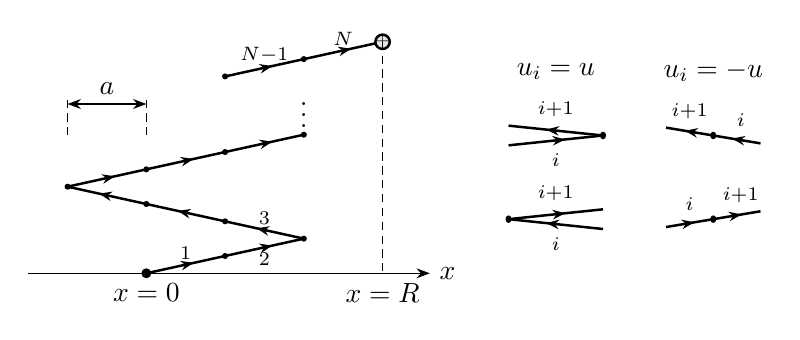
\begin{tikzpicture}[>=Stealth,line width=0.9pt,
  rod/.style={postaction={decorate},decoration={markings,mark=at position 0.6 with {\arrow{Stealth[length=1.6mm]}}}}]
  % 左：1次元高分子モデルの構造
  \draw[line width=0.4pt,->] (-1.5,0) -- (3.6,0) node[right] {$x$};
  \node[below] at (0,0) {$x=0$};
  \node[below] at (3,0) {$x=R$};
  \foreach \s/\e/\l/\p in {
    {(0,0)}/{(1,0.22)}/1/above, {(1,0.22)}/{(2,0.44)}/2/below,
    {(2,0.44)}/{(1,0.66)}/3/above, {(1,0.66)}/{(0,0.88)}//above,
    {(0,0.88)}/{(-1,1.1)}//above, {(-1,1.1)}/{(0,1.32)}//above,
    {(0,1.32)}/{(1,1.54)}//above, {(1,1.54)}/{(2,1.76)}//above}
    {\draw[rod] \s -- node[\p,inner sep=1.5pt] {\scriptsize $\l$} \e; \fill \e circle (1.1pt);}
  \fill (0,0) circle (1.8pt);
  \node at (2,2.12) {$\vdots$};
  \draw[rod] (1,2.5) -- node[above,inner sep=1.5pt] {\scriptsize $N{-}1$} (2,2.72);
  \draw[rod] (2,2.72) -- node[above,inner sep=1.5pt] {\scriptsize $N$} (3,2.94);
  \fill (1,2.5) circle (1.1pt); \fill (2,2.72) circle (1.1pt);
  \draw[fill=black!10] (3,2.94) circle (2.6pt); \node[scale=0.6] at (3,2.94) {$+$};
  \draw[line width=0.4pt,densely dashed] (3,2.94) -- (3,0);
  \draw[line width=0.4pt,densely dashed] (-1,1.75) -- (-1,2.25); \draw[line width=0.4pt,densely dashed] (0,1.75) -- (0,2.25);
  \draw[line width=0.4pt,<->] (-1,2.15) -- node[above] {$a$} (0,2.15);

  % 右：連結部分のエネルギー
  \begin{scope}[xshift=4.6cm,yshift=0.5cm,yscale=1.25]
    \node at (0.6,1.65) {$u_i=u$};
    \draw[rod] (0,0.9) -- (1.2,1.0); \draw[rod] (1.2,1.0) -- (0,1.1); \fill (1.2,1.0) circle (1.1pt);
    \node[below] at (0.6,0.92) {\scriptsize $i$}; \node[above] at (0.6,1.08) {\scriptsize $i{+}1$};
    \draw[rod] (1.2,0.05) -- (0,0.15); \draw[rod] (0,0.15) -- (1.2,0.25); \fill (0,0.15) circle (1.1pt);
    \node[below] at (0.6,0.07) {\scriptsize $i$}; \node[above] at (0.6,0.23) {\scriptsize $i{+}1$};

    \node at (2.6,1.65) {$u_i=-u$};
    \draw[rod] (3.2,0.92) -- (2.6,1.0); \draw[rod] (2.6,1.0) -- (2.0,1.08); \fill (2.6,1.0) circle (1.1pt);
    \node[above] at (2.95,0.98) {\scriptsize $i$}; \node[above] at (2.3,1.06) {\scriptsize $i{+}1$};
    \draw[rod] (2.0,0.07) -- (2.6,0.15); \draw[rod] (2.6,0.15) -- (3.2,0.23); \fill (2.6,0.15) circle (1.1pt);
    \node[above] at (2.3,0.13) {\scriptsize $i$}; \node[above] at (2.95,0.21) {\scriptsize $i{+}1$};
  \end{scope}
\end{tikzpicture}
\end{document}
